\newpage
\begin{flushleft}
  \textbf{\large 4 Проведение экспериментальной апробации}
\end{flushleft}
\refstepcounter{chapter}
\addcontentsline{toc}{chapter}{4 Проведение экспериментальной апробации}
В этой главе для всестороннего анализа качества работы алгоритмов на основе показаний метрик MOTA, HOTA и IDF1 и производительности будут описаны и проведены следующие эксперименты:
\begin{itemize}
  \item[--] исследование влияния размера сети детектора;
  \item[--] исследование влияния различных ReID моделей;
  \item[--] исследование влияния частоты кадров видеоизображения;
  \item[--] исследование влияния количества отслеживаемых объектов на производительность.
\end{itemize}


\section{Исследование зависимости показателей качества от размера сети детектора}
Первым экспериментом было решено провести сравнения показателей метрик HOTA, MOTA и IDF1 от размера сети детектора на двух различных размерах изображений. Это исследование поможет определить, насколько значителен вклад увеличения сети детектора и размера изображения. 

Для проведения экспериментов было произведено вычисление показателей качества на наборе данных MOT17 с различными конфигурациями. Результаты исследования представлены на рисунках \ref{fig:yolo_ByteTrack}-\ref{fig:yolo_ImprAssOC}.

По графикам видно, что в целом самая маленькая модель yolov8n на размере изображения 512 на 512 работает по качеству сопоставимо с самой большой yolov8x на размере изображений 312 на 312. 
Более точно числа представлены для сравнения в таблицах \ref{tab:mean_hota_yolo_size} - \ref{tab:mean_idf1_yolo_size}.

\begin{figure}[ht]
    \centering
    \includegraphics[width=1\textwidth]{plots/yolo_size_vs_metric/ByteTrack.png}
    \caption{График зависимости метрик HOTA, MOTA и IDF1 от размера сети детектора для алгоритма ByteTrack}
    \label{fig:yolo_ByteTrack}
\end{figure}

\begin{figure}[ht]
    \centering
    \includegraphics[width=1\textwidth]{plots/yolo_size_vs_metric/OC-SORT.png}
    \caption{График зависимости метрик HOTA, MOTA и IDF1 от размера сети детектора для алгоритма OC-SORT}
    \label{fig:yolo_OC-SORT}
\end{figure}

\begin{figure}[ht]
    \centering
    \includegraphics[width=1\textwidth]{plots/yolo_size_vs_metric/Deep OC-SORT.png}
    \caption{График зависимости метрик HOTA, MOTA и IDF1 от размера сети детектора для алгоритма Deep OC-SORT}
    \label{fig:yolo_Deep OC-SORT}
\end{figure}

\begin{figure}[ht]
    \centering
    \includegraphics[width=1\textwidth]{plots/yolo_size_vs_metric/StrongSORT.png}
    \caption{График зависимости метрик HOTA, MOTA и IDF1 от размера сети детектора для алгоритма StrongSORT}
    \label{fig:yolo_StrongSORT}
\end{figure}

\begin{figure}[ht]
    \centering
    \includegraphics[width=1\textwidth]{plots/yolo_size_vs_metric/BoT-SORT.png}
    \caption{График зависимости метрик HOTA, MOTA и IDF1 от размера сети детектора для алгоритма BoT-SORT}
    \label{fig:yolo_BoT-SORT}
\end{figure}

\begin{figure}[ht]
    \centering
    \includegraphics[width=1\textwidth]{plots/yolo_size_vs_metric/ImprAssOC.png}
    \caption{График зависимости метрик HOTA, MOTA и IDF1 от размера сети детектора для алгоритма ImprAssOC}
    \label{fig:yolo_ImprAssOC}
\end{figure}
\FloatBarrier
\begin{table}[htbp]

\caption{Среднее значение метрики HOTA для yolov8n и yolov8x}
\label{tab:mean_hota_yolo_size}
\centering
\begin{tabular}{lrrrr}
 & \multicolumn{2}{c}{320} & \multicolumn{2}{c}{512} \\
  & yolov8n & yolov8x & yolov8n & yolov8x \\
\midrule
BoT-SORT & 32.8 & 38.1 & 37.6 & 41.7 \\
ByteTrack & 31.0 & 35.2 & 35.2 & 38.2 \\
Deep OC-SORT & 30.6 & 35.1 & 35.4 & 38.9 \\
ImprAssOC & 34.0 & 38.3 & 38.8 & 42.0 \\
OC-SORT & 28.8 & 33.2 & 33.7 & 37.0 \\
StrongSORT & 34.5 & 39.3 & 38.9 & 42.7 \\
\bottomrule
\end{tabular}\end{table}
\begin{table}[htbp]

\caption{Среднее значение метрики MOTA для yolov8n и yolov8x}
\label{tab:mean_mota_yolo_size}
\centering
\begin{tabular}{lrrrr}
 & \multicolumn{2}{c}{320} & \multicolumn{2}{c}{512} \\
  & yolov8n & yolov8x & yolov8n & yolov8x \\
\midrule
BoT-SORT & 33.5 & 41.4 & 40.6 & 45.8 \\
ByteTrack & 32.2 & 38.2 & 37.5 & 41.2 \\
Deep OC-SORT & 31.1 & 37.9 & 37.6 & 42.0 \\
ImprAssOC & 36.2 & 44.1 & 43.3 & 48.5 \\
OC-SORT & 28.0 & 34.9 & 34.6 & 38.5 \\
StrongSORT & 34.0 & 41.1 & 40.5 & 45.5 \\
\bottomrule
\end{tabular}\end{table}
\begin{table}[htbp]

\caption{Среднее значение метрики IDF1 для yolov8n и yolov8x}
\label{tab:mean_idf1_yolo_size}
\centering
\begin{tabular}{lrrrr}
 & \multicolumn{2}{c}{320} & \multicolumn{2}{c}{512} \\
  & yolov8n & yolov8x & yolov8n & yolov8x \\
\midrule
BoT-SORT & 43.7 & 50.6 & 50.0 & 55.4 \\
ByteTrack & 40.9 & 46.3 & 45.9 & 49.8 \\
Deep OC-SORT & 40.7 & 46.5 & 46.9 & 51.7 \\
ImprAssOC & 44.3 & 48.9 & 50.2 & 53.7 \\
OC-SORT & 37.1 & 43.1 & 43.5 & 47.6 \\
StrongSORT & 47.0 & 53.3 & 52.6 & 57.6 \\
\bottomrule
\end{tabular}\end{table}
\FloatBarrier


\section{Исследование зависимости показателей качества от размера ReID модели}
Вторым экспериментом было проведение сравнения результатом для различных ReID моделей. Благодаря этому, можно будет понять, насколько использование более требовательных моделей оправдано. 

В ходе эксперимента, для каждой сети детектора и размера изображения из прошлого пункта был проведен анализ точности работы отдельных ReID моделей на наборе данных MOT17. Полученные результаты можно увидеть на рисунках \ref{fig:yolo_reid_ByteTrack}-\ref{fig:yolo_reid_ImprAssOC}. Отдельно стоит отметить, что на рисунках \ref{fig:yolo_reid_ByteTrack}-\ref{fig:yolo_reid_OC-SORT} нет влияния выбора, так как реализации алгоритмом ByteTrack и OC-SORT не используют ReID модели, а основываются на метрике IoU.

Полученные графики явно показывают, что только самая маленькая ReID модель OSNet x0.25 дает стабильно более низкий результат. При этом все остальные модели дают абсолютно схожие показатели с минимальными улучшениями относительно друг друга.
\begin{figure}[ht]
    \centering
    \includegraphics[width=1\textwidth]{plots/yolo_size_and_reid_vs_metric/ByteTrack.png}
    \caption{График зависимости метрик HOTA, MOTA и IDF1 от ReID модели для алгоритма ByteTrack}
    \label{fig:yolo_reid_ByteTrack}
\end{figure}

\begin{figure}[ht]
    \centering
    \includegraphics[width=1\textwidth]{plots/yolo_size_and_reid_vs_metric/OC-SORT.png}
    \caption{График зависимости метрик HOTA, MOTA и IDF1 от ReID модели для алгоритма OC-SORT}
    \label{fig:yolo_reid_OC-SORT}
\end{figure}

\begin{figure}[ht]
    \centering
    \includegraphics[width=1\textwidth]{plots/yolo_size_and_reid_vs_metric/Deep OC-SORT.png}
    \caption{График зависимости метрик HOTA, MOTA и IDF1 от ReID модели для алгоритма Deep OC-SORT}
    \label{fig:yolo_reid_Deep OC-SORT}
\end{figure}

\begin{figure}[ht]
    \centering
    \includegraphics[width=1\textwidth]{plots/yolo_size_and_reid_vs_metric/StrongSORT.png}
    \caption{График зависимости метрик HOTA, MOTA и IDF1 от ReID модели для алгоритма StrongSORT}
    \label{fig:yolo_reid_StrongSORT}
\end{figure}

\begin{figure}[ht]
    \centering
    \includegraphics[width=1\textwidth]{plots/yolo_size_and_reid_vs_metric/BoT-SORT.png}
    \caption{График зависимости метрик HOTA, MOTA и IDF1 от ReID модели для алгоритма BoT-SORT}
    \label{fig:yolo_reid_BoT-SORT}
\end{figure}

\begin{figure}[ht]
    \centering
    \includegraphics[width=1\textwidth]{plots/yolo_size_and_reid_vs_metric/ImprAssOC.png}
    \caption{График зависимости метрик HOTA, MOTA и IDF1 от ReID модели для алгоритма ImprAssOC}
    \label{fig:yolo_reid_ImprAssOC}
\end{figure}
\FloatBarrier

% TODO: можно добавить сравнения на низких фпс табличку, там вроде то же самое, но для объема

\section{Исследование зависимости показателей качества от частоты кадров видеоизображения}
В ходе работы также было проведено исследование зависимости показателей качества от частоты кадров видеоизображения. 
Мотивация этого сравнения заключается в том, что при запуске на микрокомпьютере скорость работы заметно ниже, а значит временные промежутки между кадрами больше. 
В следствии этого, объекты на изображении будут перемещаться сильнее между кадрами, что повлияет на качество отслеживания. 
Именно поэтому, для адекватного сравнения алгоритмов между собой, важно пересчитать метрики для разных показателей частоты кадров. 

На рисунках \ref{fig:fps_ByteTrack}-\ref{fig:fps_ImprAssOC} виден результат проведенного сравнения. 
Все показатели медианные для каждого алгоритма. 
Для анализа выбраны детекторы yolov8n и yolov8s, так как только они способны запускаться на микрокомпьютере с частотой кадров больше 10, а также yolov8x как эталон возможного максимума.
Частоты кадров видеоизображения для сравнения подобраны методом кластеризации k-средних всех полученных результатов частоты работы на микрокомпьютере.
По результатам эксперимента получена таблица \ref{tab:correlation_hota_fpsbench_tracker}. 
\begin{table}[htbp]
\caption{Корреляция метрики HOTA с частотой кадров видеоизображения}
\label{tab:correlation_hota_fpsbench_tracker}
\centering
\begin{tabular}{lrr}
\toprule
Частота & (0, 6] & [6, 30] \\
кадров, Гц &  &  \\
\midrule
BoT-SORT & 0.91 & 0.21 \\
ByteTrack & 0.93 & 0.44 \\
Deep OC-SORT & 0.91 & 0.36 \\
ImprAssOC & 0.71 & 0.36 \\
OC-SORT & 0.92 & 0.48 \\
StrongSORT & 0.89 & 0.16 \\
\bottomrule
\end{tabular}

\end{table}

\begin{figure}[ht]
    \centering
    \includegraphics[width=1\textwidth]{plots/fps_vs_metric/ByteTrack.png}
    \caption{График зависимости метрик HOTA, MOTA и IDF1 от частоты кадров видеоизображения для алгоритма ByteTrack}
    \label{fig:fps_ByteTrack}
\end{figure}

\begin{figure}[ht]
    \centering
    \includegraphics[width=1\textwidth]{plots/fps_vs_metric/OC-SORT.png}
    \caption{График зависимости метрик HOTA, MOTA и IDF1 от частоты кадров видеоизображения для алгоритма OC-SORT}
    \label{fig:fps_OC-SORT}
\end{figure}

\begin{figure}[ht]
    \centering
    \includegraphics[width=1\textwidth]{plots/fps_vs_metric/Deep OC-SORT.png}
    \caption{График зависимости метрик HOTA, MOTA и IDF1 от частоты кадров видеоизображения для алгоритма Deep OC-SORT}
    \label{fig:fps_Deep OC-SORT}
\end{figure}

\begin{figure}[ht]
    \centering
    \includegraphics[width=1\textwidth]{plots/fps_vs_metric/StrongSORT.png}
    \caption{График зависимости метрик HOTA, MOTA и IDF1 от частоты кадров видеоизображения для алгоритма StrongSORT}
    \label{fig:fps_StrongSORT}
\end{figure}

\begin{figure}[ht]
    \centering
    \includegraphics[width=1\textwidth]{plots/fps_vs_metric/BoT-SORT.png}
    \caption{График зависимости метрик HOTA, MOTA и IDF1 от частоты кадров видеоизображения для алгоритма BoT-SORT}
    \label{fig:fps_BoT-SORT}
\end{figure}

\begin{figure}[ht]
    \centering
    \includegraphics[width=1\textwidth]{plots/fps_vs_metric/ImprAssOC.png}
    \caption{График зависимости метрик HOTA, MOTA и IDF1 от частоты кадров видеоизображения для алгоритма ImprAssOC}
    \label{fig:fps_ImprAssOC}
\end{figure}
\FloatBarrier

По полученным результатам четко видна общая закономерность почти для всех методов: 
\begin{itemize}
    \item до 5 кадров в секунду идет значительный линейный рост показателей метрик HOTA, MOTA и IDF1;
    \item с 5 до 11 происходит небольшое улучшение;
    \item при частоте выше 11 показатели или выходят на плато, или растут незначительно.
\end{itemize}
Вероятно, плато является следствием увеличения шумов с ростом частоты кадров видеоизображения, так как перемещения между кадрами становятся все меньше и меньше, а погрешность детектора в несколько пикселей начинает играть все большую роль и перевешивает плюсы от меньших перемещений.

\section{Исследование зависимости производительности от количества объектов на видеоизображении}
При большом количестве объектов на изображении происходит ощутимая просадка частоты работы при использовании алгоритмов с ReID моделями. 
Это связано с тем, что их вычисления невозможно перенести на TPU в связи с произвольным размером входа сети.  
Четвертым экспериментом было решено провести исследование величин этих просадок. Для этого было сделано видео, где на черном фоне один за одним с интервалом в секунду появляются объекты. 
Результаты запуска различных конфигураций алгоритмов представлены на рисунках \ref{fig:fps_object_ByteTrack}-\ref{fig:fps_object_ImprAssOC}.

По результатам эксперимента получена таблица получена таблица \ref{tab:correlation_fps_object}. 
\begin{table}[htbp]
\caption{Корреляция частоты работы с количеством объектов на изображении}
\label{tab:correlation_fps_object}
\centering
\begin{tabular}{lr}
\toprule
Алгоритм & Корреляция \\
\midrule
BoT-SORT & -0.63 \\
ByteTrack & -0.03 \\
Deep OC-SORT & -0.65 \\
ImprAssOC & -0.63 \\
OC-SORT & -0.10 \\
StrongSORT & -0.66 \\
\bottomrule
\end{tabular}

\end{table}
ByteTrack и OC-SORT -- два алгоритма не использующие ReID-модели -- наименее чувствительные к увеличению количества отслеживаемых объектов.
\begin{figure}[ht]
    \centering
    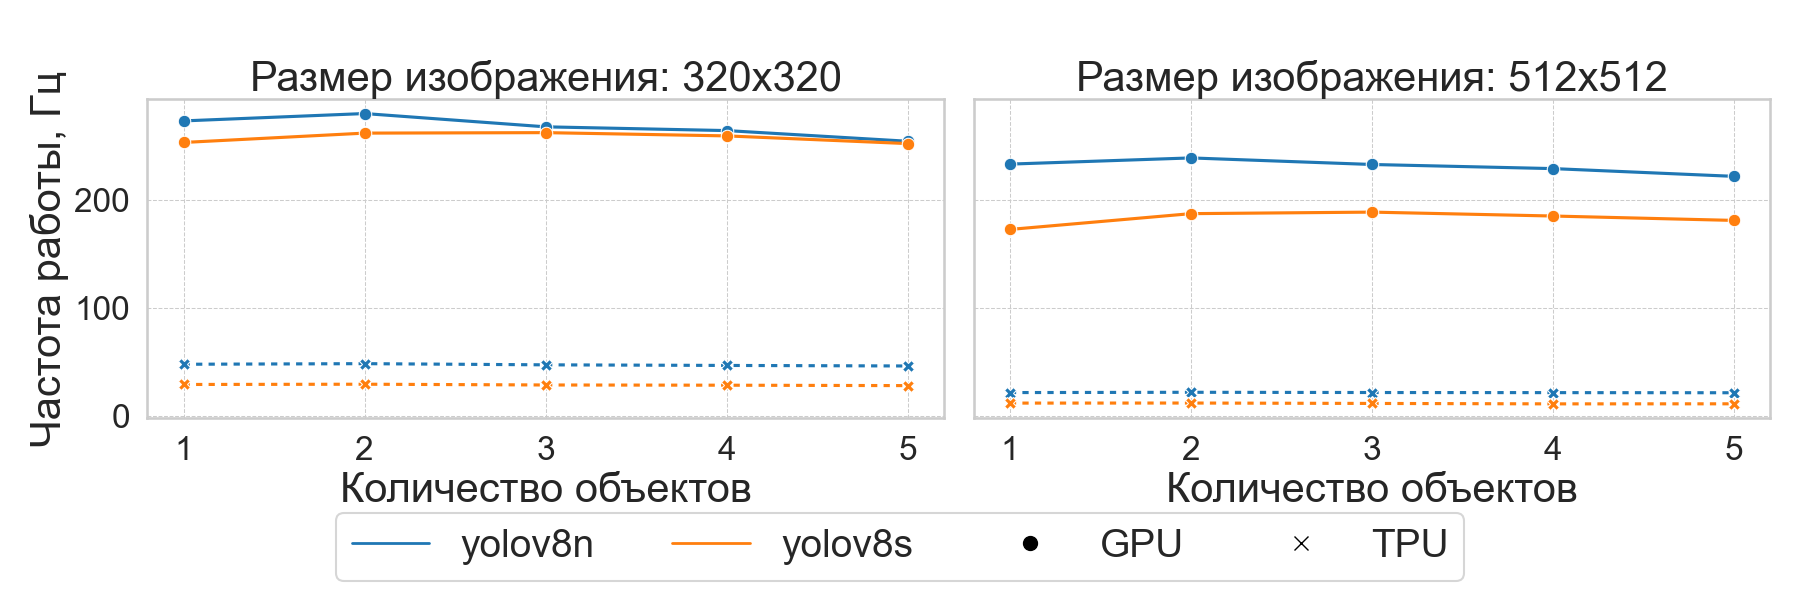
\includegraphics[width=1\textwidth]{plots/fps_vs_object_count/ByteTrack_gpu_tpu.png}
    \caption{График зависимости частоты работы алгоритма ByteTrack от количества объектов на изображении}
    \label{fig:fps_object_ByteTrack}
\end{figure}

\begin{figure}[ht]
    \centering
    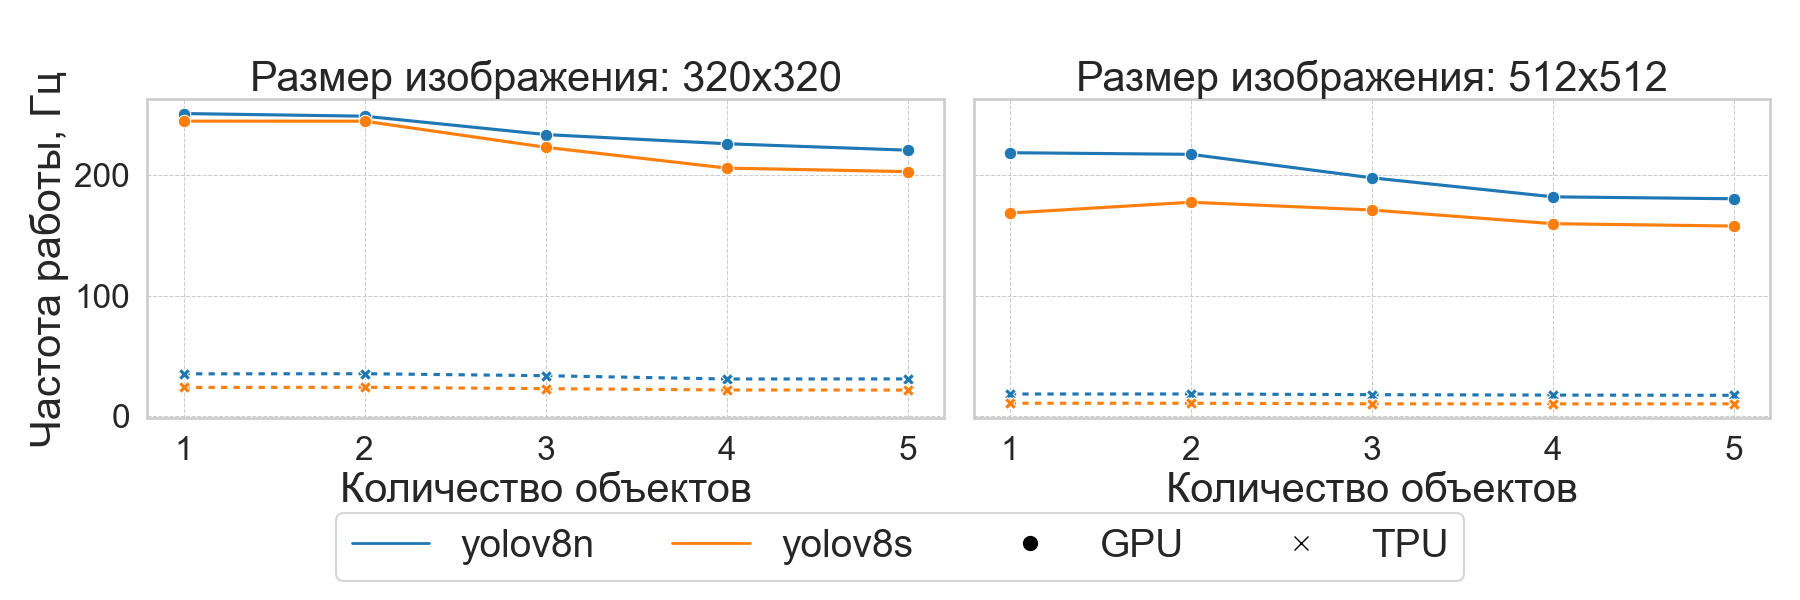
\includegraphics[width=1\textwidth]{plots/fps_vs_object_count/OC-SORT_gpu_tpu.png}
    \caption{График зависимости частоты работы алгоритма OC-SORT от количества объектов на изображении}
    \label{fig:fps_object_OC-SORT}
\end{figure}

\begin{figure}[ht]
    \centering
    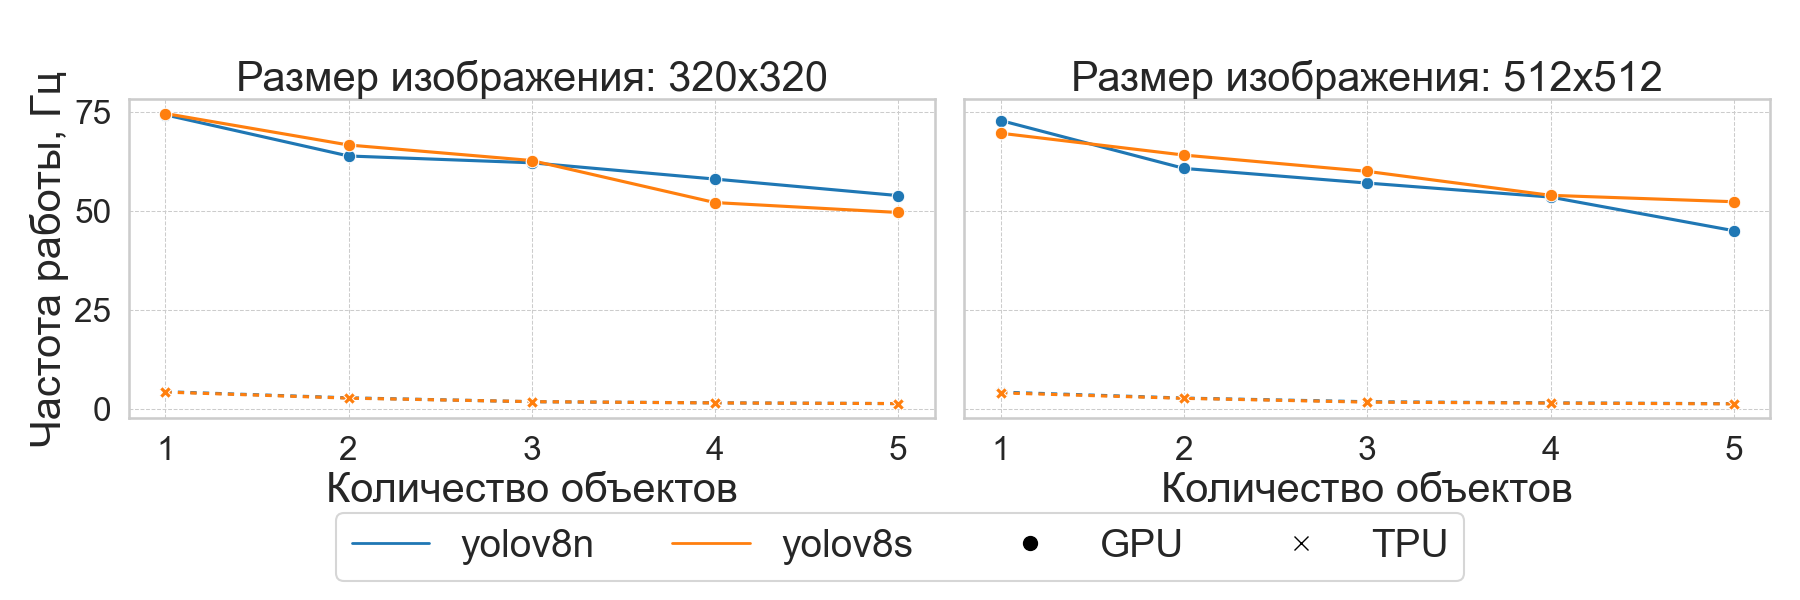
\includegraphics[width=1\textwidth]{plots/fps_vs_object_count/Deep OC-SORT_gpu_tpu.png}
    \caption{График зависимости частоты работы алгоритма Deep OC-SORT от количества объектов на изображении}
    \label{fig:fps_object_Deep OC-SORT}
\end{figure}

\begin{figure}[ht]
    \centering
    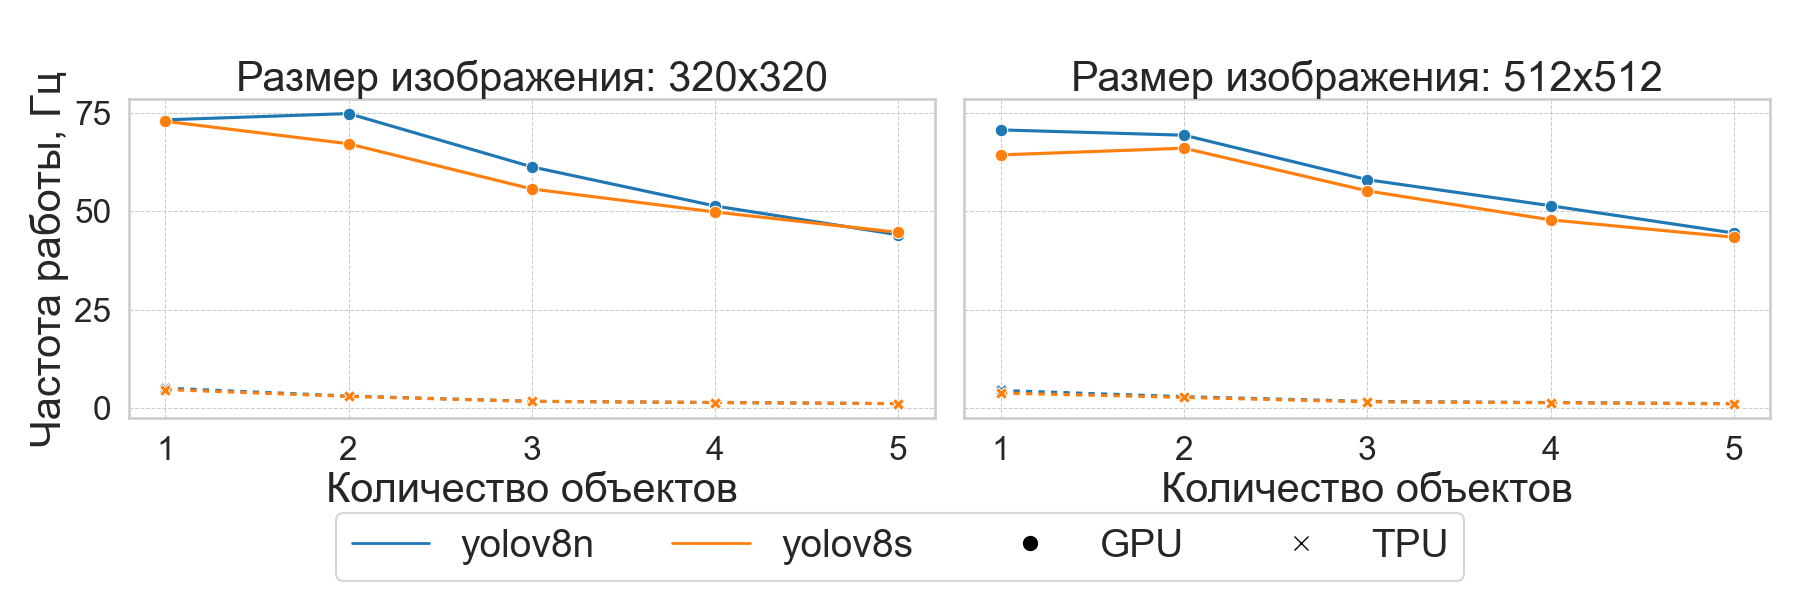
\includegraphics[width=1\textwidth]{plots/fps_vs_object_count/StrongSORT_gpu_tpu.png}
    \caption{График зависимости частоты работы алгоритма StrongSORT от количества объектов на изображении}
    \label{fig:fps_object_StrongSORT}
\end{figure}

\begin{figure}[ht]
    \centering
    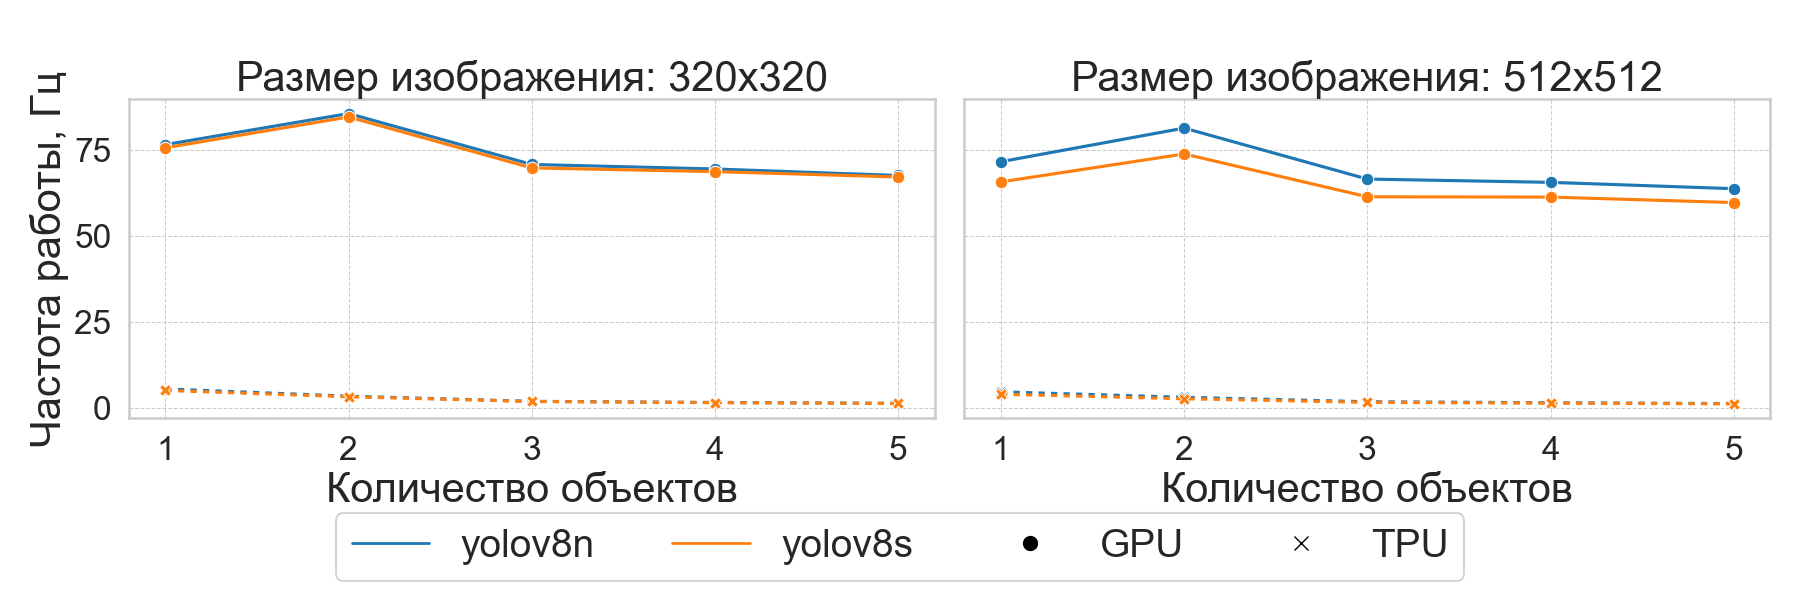
\includegraphics[width=1\textwidth]{plots/fps_vs_object_count/BoT-SORT_gpu_tpu.png}
    \caption{График зависимости частоты работы алгоритма BoT-SORT от количества объектов на изображении}
    \label{fig:fps_object_BoT-SORT}
\end{figure}

\begin{figure}[ht]
    \centering
    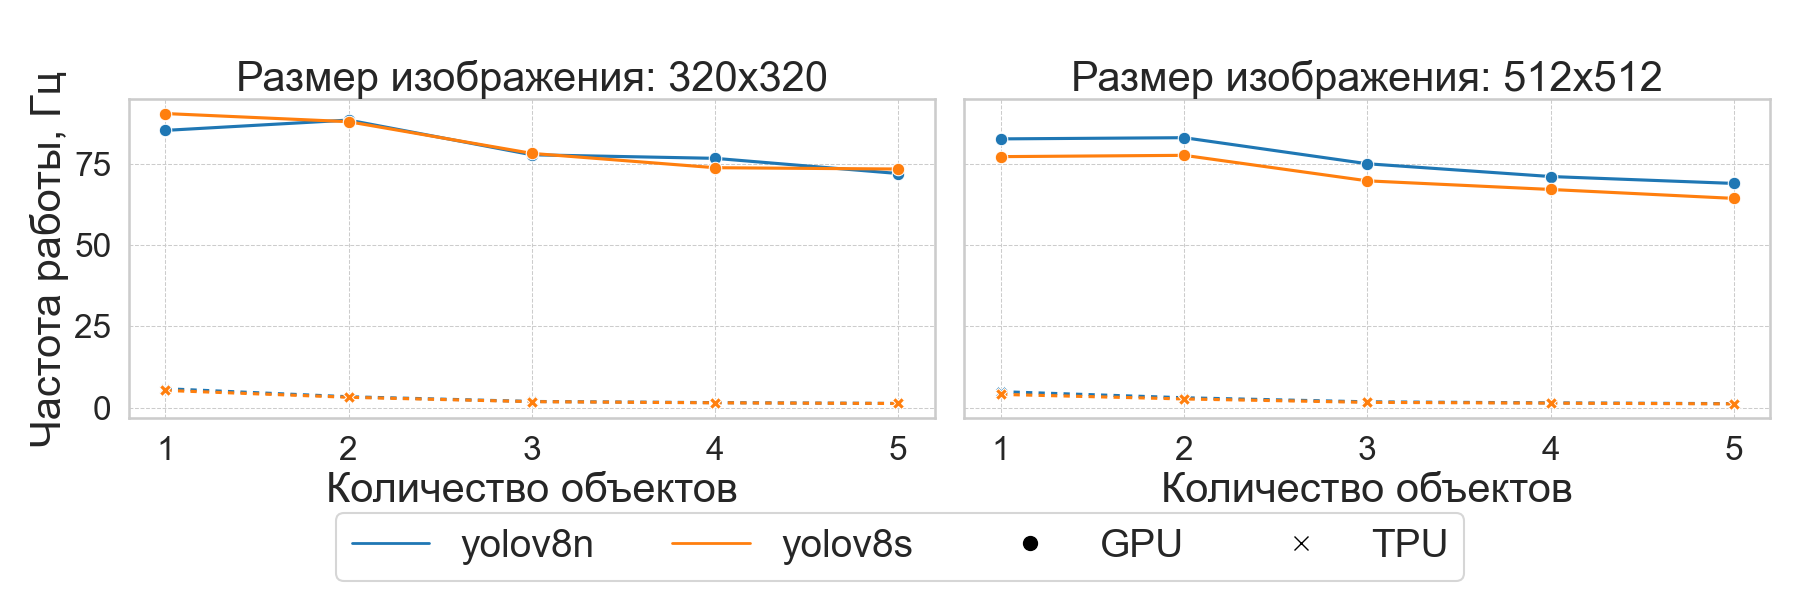
\includegraphics[width=1\textwidth]{plots/fps_vs_object_count/ImprAssOC_gpu_tpu.png}
    \caption{График зависимости частоты работы алгоритма ImprAssOC от количества объектов на изображении}
    \label{fig:fps_object_ImprAssOC}
\end{figure}
\FloatBarrier

\section{Выводы по главе}
Результаты всех экспериментов были сведены в таблицы, представленные на рисунках \ref{fig:fps_hota_n320}-\ref{fig:fps_hota_s512} на каждом из которых две таблицы: первая содержит данные о скорости работы различных сочетаний алгоритмов с ReID-моделями на Raspberry Pi 5 с Google Coral TPU; вторая -- показатель метрики качества HOTA. 

\begin{figure}[ht]
  \centering
  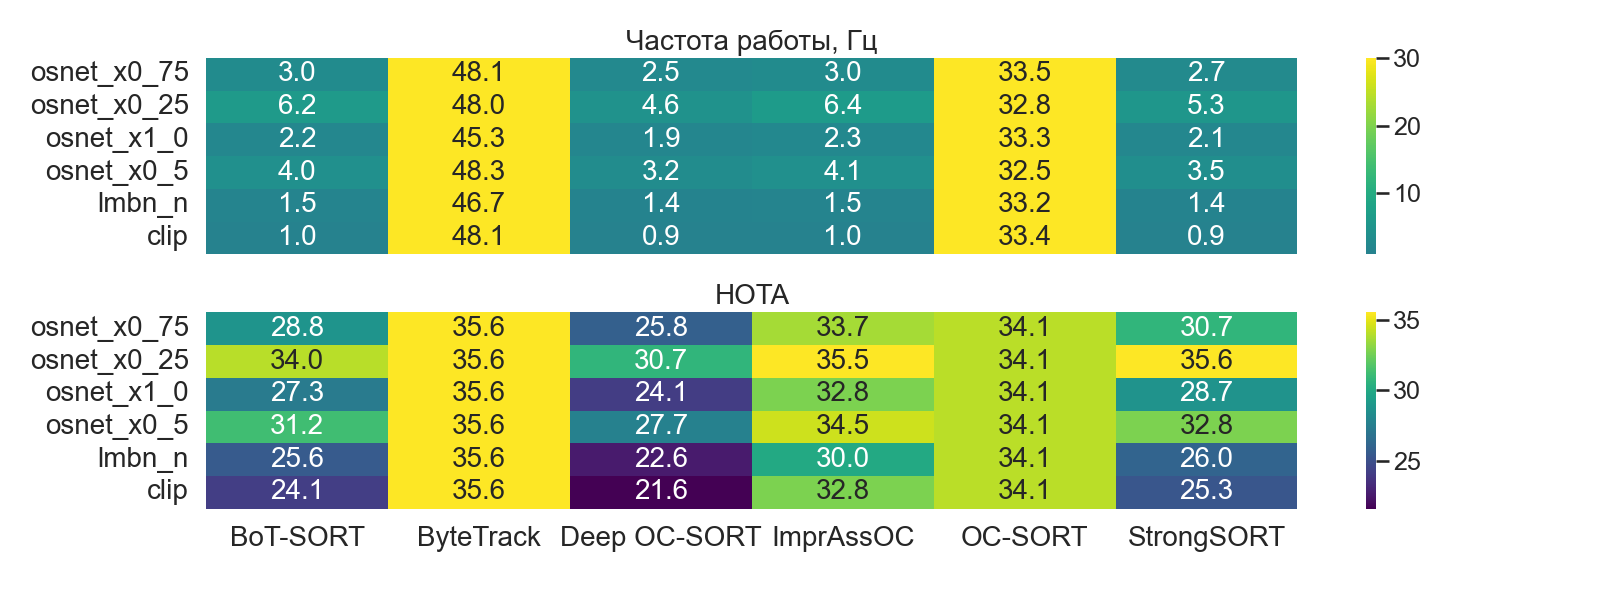
\includegraphics[width=1\textwidth]{./plots/heatmap_fps_hota_vs_tracker_reid/heatmap_fps_hota_yolov8n_size320.png}
  \caption{Таблица производительности и метрики HOTA для yolov8n с размером изображения 320}
  \label{fig:fps_hota_n320}
\end{figure}

\begin{figure}[ht]
  \centering
  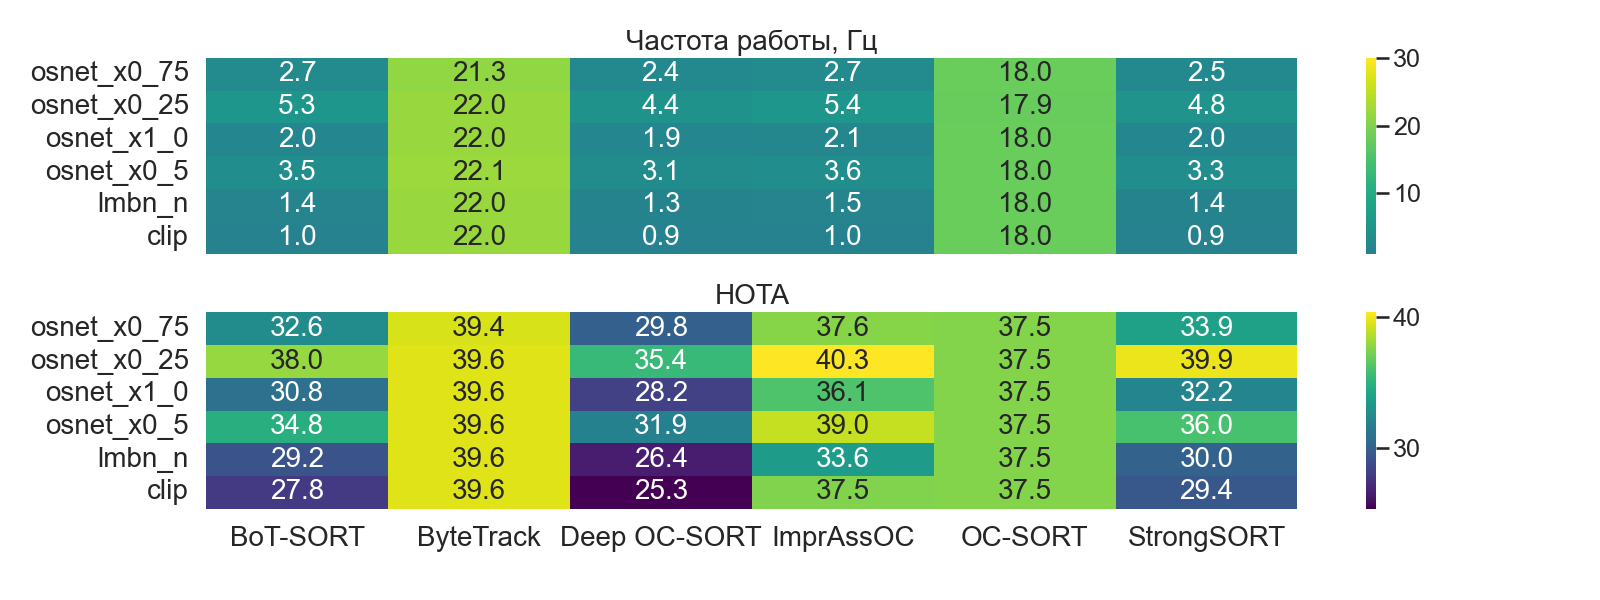
\includegraphics[width=1\textwidth]{./plots/heatmap_fps_hota_vs_tracker_reid/heatmap_fps_hota_yolov8n_size512.png}
  \caption{Таблица производительности и метрики HOTA для yolov8n с размером изображения 512}
  \label{fig:fps_hota_n512}
\end{figure}


\begin{figure}[ht]
  \centering
  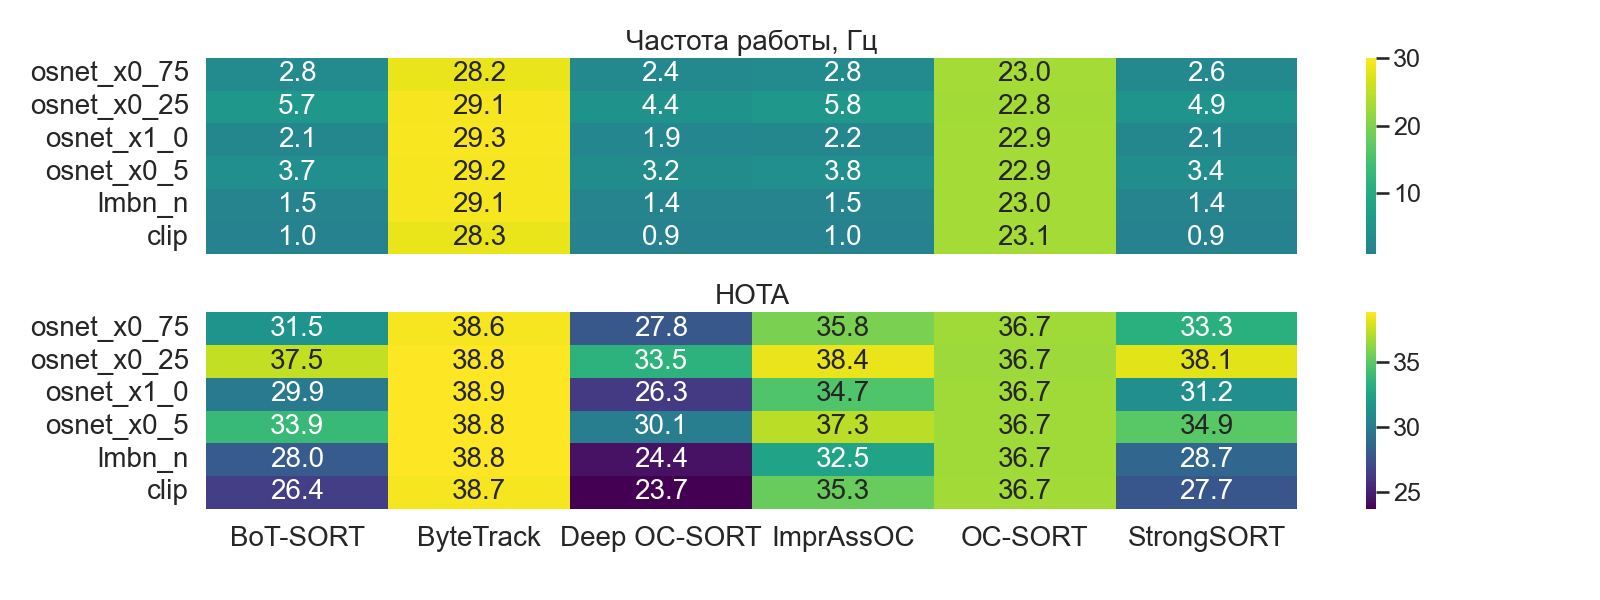
\includegraphics[width=1\textwidth]{./plots/heatmap_fps_hota_vs_tracker_reid/heatmap_fps_hota_yolov8s_size320.png}
  \caption{Таблица производительности и метрики HOTA для yolov8s с размером изображения 320}
  \label{fig:fps_hota_s320}
\end{figure}

\begin{figure}[ht]
  \centering
  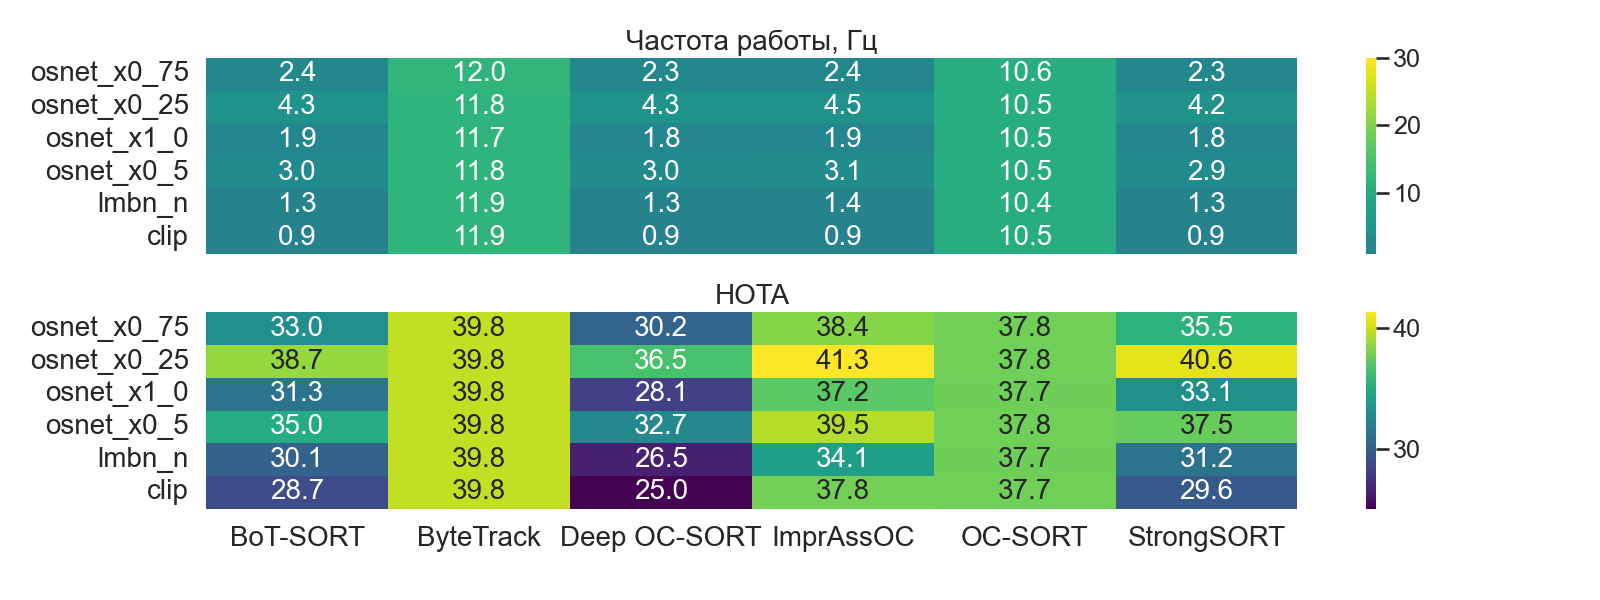
\includegraphics[width=1\textwidth]{./plots/heatmap_fps_hota_vs_tracker_reid/heatmap_fps_hota_yolov8s_size512.png}
  \caption{Таблица производительности и метрики HOTA для yolov8s с размером изображения 512}
  \label{fig:fps_hota_s512}
\end{figure}
\FloatBarrier
